\documentclass[12pt]{article}
\usepackage{amsmath,amsthm,amssymb,amsfonts,fullpage,verbatim,bm,graphicx,enumerate,epstopdf,lscape,enumitem}
\usepackage[titletoc,title]{appendix}
\usepackage[dvipsnames,usenames]{color}
\usepackage[pdftex,pagebackref,colorlinks=true,pdfpagemode=UseNone,urlcolor=blue,linkcolor=blue,citecolor=BrickRed,pdfstartview=FitH,plainpages=true]{hyperref}
\usepackage[top=1.15in,bottom=1.15in,left=1.25in,right=1.25in,letterpaper]{geometry}
\usepackage[font=scriptsize]{caption}
\usepackage{caption,subcaption}

\setlist{noitemsep}

\def\CC{\mathbb{C}}
\def\RR{\mathbb{R}}
\def\ZZ{\mathbb{Z}}
\def\PP{\mathbb{P}}
\def\EE{\mathbb{E}}
\def\II{\mathbb{I}}


\newcommand{\Ga}{\alpha}
\newcommand{\Gb}{\beta}
\newcommand{\Gg}{\gamma}     \newcommand{\GG}{\Gamma}
\newcommand{\Gd}{\delta}     \newcommand{\GD}{\Delta}
\newcommand{\Ge}{\epsilon}
\newcommand{\Gf}{\phi}       \newcommand{\GF}{\Phi}
\newcommand{\Gh}{\theta}
\newcommand{\Gi}{\iota}
\newcommand{\Gk}{\kappa}
\newcommand{\Gl}{\lambda}    \newcommand{\GL}{\Lambda}
\newcommand{\Go}{\omega}     \newcommand{\GO}{\Omega}
\newcommand{\Gs}{\sigma}     \newcommand{\GS}{\Sigma}
\newcommand{\Gt}{\tau}
\newcommand{\Gz}{\zeta}
\newcommand{\s}{\sigma}
\newcommand{\tr}{\triangle}


\begin{document}

\title{\textbf{Title}}
\date{}
\maketitle

\section{Abstract}
\section{Introduction}
In recent years, the use of various shrinkage and thresholding procedures has become ever more popular in a variety of applications where sparsity is a desirable notion. Here the term ``sparsity'' is loosely defined in the sense that it also includes the case where there are many near-zero (as opposed to exactly zero) terms, as shrinkage procedures often produce. The most prominent usage of such procedures appear in multiresolution denoising analyses such as wavelets, where sparsity in a transformed domain often corresponds to smoothness in the data space [references]. Other examples include estimation of covariance and precision matrices (though thresholding is used more often here since zero terms are usually desired) [references], accounting for different measurement precisions in FDR control for multiple testing [references], or more generally optimizing penalized likelihood problems such as LASSO [references]. In this paper we will look at a flexible and adaptive shrinkage method named ASH, and illustrate its value in two key areas of univariate wavelet denoising.\bigskip\\
Before delving deeper into the two denoising tasks, we first present a brief overview of wavelet estimators. These estimators have become extremely popular in nonparametric regression problems following the seminal paper by Donoho \& Johnstone (1994). Not only are wavelet methods locally adaptive in the sense that they achieve the optimal minimax rate over a wide variety of functions, but they are also computationally faster than many other adaptive methods such as variable-bandwidth kernel methods [antoniadis 2001]. While classical thresholding estimators have been shown to possess optimal asymptotic properties, an extensive simulation study by Antoniadis et al. (2001) has demonstrated that various Bayesian shrinkage methods can often outperform thresholding methods in finite samples, where performance is measured by mean squared error (MSE). However, many existing Bayesian wavelet methods are often computationally intensive, and may not be practical for large scale applications. Furthermore, it is not easy to apply the same thresholding or Bayesian shrinkage rules to other nonparametric regression problems, two of which we subsequently describe. On the other hand, our method is computationally faster than previous Bayesian methods while still possessing good finite sample performance, and use ASH as the common shrinkage procedure in both the problems.\bigskip\\
The first problem relates to the frequently encountered Gaussian case. Although the theory for mean estimation with homoskedastic Gaussian errors has been thoroughly developed in the wavelet literature [references], the existing methods for variance estimation with heteroskedastic errors have been far and few between. Fan \& Yao (1998) estimated the variance by smoothing the squared residuals using local polynomial smoothing, while Brown \& Levine (2007) employed difference-based kernel estimators. Making use of the local adaptivity of wavelet methods, Cai \& Wang (2008) improved upon previous approaches using a wavelet thresholding approach on first order differences. While Cai \& Wang (2008) proved that their technique was asymptotically optimal, we will demonstrate how we can further improve the finite sample performance of previous variance estimation procedures by incorporating ASH into a novel wavelet denoising framework. [mention the lack of available software?]\bigskip\\
The second task is to denoise a Poisson distributed signal. This often occurs in the experimental sciences such as gamma-ray burst signals in astronomy [references], and more recently in genetics where high throughput sequencing data is of interest. This problem is particularly interesting in the sense that there are many different ways to perform signal recovery. Variance stabilizing techniques together with normal approximations have been proposed by Donoho (1993) and Fryzlewicz \& Nason (2001), by noting that the variance of a Poisson count is equal to its mean. Kolaczyk (1997, 1999a) derived thresholds achieving optimal asymptotic properties in the context of wavelet transformations, similar to the thresholds in the i.i.d. Gaussian case.  However, variance stabilizing methods are computationally inefficient due to the presence of external cycle-spinning, and threshold-based methods may not result in optimal finite sample performance. Furthermore, both these methods are quite sensitive to the choice of the primary resolution level due to the Poisson nature of the data. Multiscale analysis using recursive dyadic partitions within a Bayesian framework was later developed by Kolaczyk (1999b) to make use of a particular form of likelihood factorization, but a relatively inflexible conjugate prior was chosen. We will improve upon the prior (and likelihood) specification by using ASH as the main shrinkage procedure in a Bayesian framework similar to that of Kolaczyk (1999b). \bigskip\\
Both these problems are generally harder to deal with than the classical problem of i.i.d. Gaussian errors, and usually requires some work in extending the ideas from methods aimed at the latter task. Before proceeding to describe the two problems in detail, we will first describe briefly the portion of ASH that performs shrinkage. \bigskip\\
As a generic shrinkage method, ASH takes as input a vector of estimates $\hat{\Gb}_i,i=1,...,n$ and their standard errors $\hat{\s}_i\equiv se(\hat{\Gb}_i),i=1,...n$, and outputs shrunken estimates of $\bm{\Gb}$. Specifically, the likelihoods for the true parameters $\Gb_i,i=1,...n$ are assumed to be iid $N(\Gb_i;\hat{\Gb}_i,\hat{\s}_i^2)$. ASH then assumes exchangeability of the $\Gb_i$'s and sets the following ``shrinkage'' prior on $\Gb_i$ for each $i$:
\begin{eqnarray}
\Gb_i|\bm{\pi}=\sum_{k=1}^m \pi_k N(\Gb_i;0,s_k^2)
\end{eqnarray}
Note that $\bm{\pi}$ and $\bm{s}^2$ is shared across all the $\Gb_i$'s, allowing one to borrow information across all the observations. The full likelihood for $\bm{\pi}$ given $\bm{\hat{\Gb}}$ and $\bm{\hat{\s}}$ is then a product of likelihoods for $\bm{\pi}$ given each $\hat{\Gb}_i$ and $\hat{\s}_i$. Since the likelihoods are Gaussian and the priors are mixtures of Gaussians, the posterior distribution of $\Gb_i$ given $\hat{\Gb}_i$ and $\bm{\hat{\pi}}$ is analytically tractable, where the mixing proportions $\bm{\hat{\pi}}$ are maximum likelihood estimates. The posterior mean of $\Gb_i$ is taken to be the point estimate of $\Gb_i$, resulting in a shrinkage procedure.\bigskip\\
The flexibility and computational efficiency of this shrinkage procedure is immediately obvious, which motivates us to extend this method to the more complex wavelet setting described here. Gaussian mixture priors can effectively approximate any unimodal distribution, allowing us to apply this single shrinkage procedure to the two problems we will be focusing on. At the same time, we can speed up the entire signal denoising problem via likelihood approximations (discussed in the next section), allowing our method to be computationally efficient without compromising too much accuracy. Furthermore, it should be noted that many wavelet methods require the specification of a primary resolution level as an extra parameter, which could substantially influence the accuracy of the method. On the other hand, we can apply ASH to every resolution in the wavelet transformation, sparing the need for such a parameter. For an in-depth understanding of the original motivations and applications of ASH, see Stephens (??). With the main shrinkage method accounted for, we will now proceed to explore the two aforementioned problems in detail. Note that one only needs to supply a vector of estimates $\hat{\Gb}$ and their standard errors se$(\hat{\Gb})$ to ASH to obtain posterior estimates; hence, we will focus on obtaining these estimates and standard errors when describing our methods.
\section{Method}
\subsection{Gaussian denoising with heteroskedastic errors}
We first consider the application of ASH in the context of the nonparametric regression model with i.i.d. Gaussian errors that are spatially structured. Specifically, consider the model
\begin{eqnarray}\label{eq:1d gaussian model}
Y_i=\mu_i+\Ge_i
\end{eqnarray}
for $i=1,...,n$, where $\bm{Y}$ is the vector of observations, $\bm{\mu}$ is the mean curve sampled on an equally spaced grid, and $\Ge_i$ are independent $N(0,\s^2)$ noise. Assume that $n=2^J$ for some integer $J$, as is standard in the wavelet literature. To better understand and motivate our method, we first look at wavelet shrinkage from a Bayesian perspective.\bigskip\\
Given an orthogonal $n\times n$ matrix $W$ representing the orthonormal wavelet basis chosen, we have that the wavelet coefficients $\bm{d}$ are given by
\begin{eqnarray}
\bm{d}=W\bm{Y}
\end{eqnarray}
where $\mathbb{V}(Y)=\s^2I$. Hence, we can easily see that
\begin{eqnarray}\label{eq:waveletcoef}
\bm{d}\sim N_n(\bm{\Ga},\s^2I)
\end{eqnarray}
where $\bm{\Ga}=W\mathbb{E}(\bm{Y})$. This implies that the likelihood for $\bm{\Ga}$ factorizes into a product of likelihoods for $\Ga_i$, $i=1,...,n$. As such, a natural and computationally convenient approach is to set independent priors on $\Ga_i$ as a form of ``shrinkage''. Here we apply the priors from ASH to each resolution level separately, resulting in
%Although there are many choices for the prior, we use the Gaussian mixture prior from ASH in our method, given by
\begin{eqnarray}\label{eq:ashprior}
\Ga_{jk}=\sum_{l=1}^m \pi_l^{(j)} N(0,(s_l^{(j)})^2)
\end{eqnarray}
with $\sum_l \pi_l^{(j)}=1$, for $j=1,...,J$. $\pi_i^{(j)}$ and $(s_i^{(j)})^2$ are hyperparameters that are shared between coefficients in the same resolution level, and $m$ is the number of mixture components. In ASH, $m$ is usually chosen so that it is large enough to reasonably approximate any unimodal distribution, while maintaining a reasonable computational speed. Note that, for notational convenience, we have switched to a double index following standard wavelet convention for indices: here $j=1,...,J$ is the resolution level, and $k=0,...,2^j-1$ is the location within each resolution level $j$. By applying the inverse wavelet transform on the posterior mean $\hat{\bm{\Ga}}$ that ASH produces, one can obtain the posterior mean of $\bm{\mu}$, which serves as an estimate that minimizes the MSE. One could also construct credible bands using the posterior variances.\bigskip\\
While many existing methods do a good job of signal denoising in the presence of i.i.d. (Gaussian) errors, heteroskedastic (but still independent) errors present a different challenge. One key obstacle when dealing with heteroskedastic errors is that the likelihood for $\bm{\Ga}$ does not necessarily factorize. If the true variances were known, one could obviously write out the full likelihood and proceed to compute the posterior mean/median using some specified prior. However, this would be computationally cumbersome, and may not be feasible when extended to multiple signals or higher dimensions. A suitable prior might also be difficult to find. As such, one key aspect of our approach is to treat the wavelet coefficients as if they were independent, so that the true likelihood is approximated by a composite likelihood (see Silverman (1999) for an example where this is done).\bigskip\\
To describe our approach in more detail, first assume that the true variance function is known and given by $\mathbb{V}(\Ge_i)=\s_i$, and that the true mean function is given by $\bm{\mu}=(\mu_1,...,\mu_t)$, where $T=2^J$ for some positive integer $J$. Hence
\begin{eqnarray}
\bm{Y}\sim N_n(\bm{\mu},\Sigma)
\end{eqnarray}
where $\Sigma=\textrm{diag}(\s_1,...,\s_T)$ is a diagonal matrix. For the rest of this subsection, we will use the non-decimated wavelet transform (NDWT) instead of the standard DWT to achieve translation invariance. This property of translation invariance reduces the presence of artifacts, which often occur near discontinuities in the underlying signal (see eg. Coifman \& Donoho (1995)). Now let $W$ be the matrix associated with the NDWT for a given wavelet basis, so that
\begin{eqnarray}
\bm{d}\sim N_n(\bm{\Ga},\tilde{\Sigma})
\end{eqnarray}
where $\bm{d}$ is the vector of detail coefficients, $\bm{\Ga}=W\bm{\mu}$, and $\tilde{\Sigma}=W\Sigma W^T$. By treating the likelihood for $\bm{\Ga}$ as if it were independent, we can write the likelihood as follows (using the double index mentioned above):
\begin{eqnarray}\label{eq:likelihood}
L(\bm{\Ga}|\bm{d})=\prod_{j=0}^J\prod_{k=0}^{T-1}P(d_{jk}|\Ga_{jk})
\end{eqnarray}
where $P(d_{jk}|\Ga_{jk})=\phi(d_{jk};\Ga_{jk},\tilde{\Sigma}_{(jk,jk)})$. Note that there are $n$ coefficients at each resolution level instead of $2^j$ for resolution $j$ because we are using the NDWT instead of the standard wavelet transform. Here $\phi$ denotes the Gaussian density function. Since $\Sigma$ is diagonal, it is easy to see that $\tilde{\Sigma}_{(jk,jk)}=\sum_{i=1}^T \Sigma_{ii}W_{jk,i}^2$. In our method, we use ASH to assign independent priors to $\Ga_{jk}$ as with \eqref{eq:ashprior}. %ASH also allows us to estimate the $\pi_i$'s via a maximum likelihood approach and fix the $\s_i$'s by using a grid of values. This particular choice of prior specification is extremely flexible, being able to approximate any symmetrical zero-centered distribution, as well as allowing for a relatively easy estimation of the hyperparameters through empirical Bayes. See ASH for more details regarding this choice of prior (?)
While ASH produces shrunken estimates of $\Ga_{jk}$ for $j,k>0$, we estimate $\Ga_{00}$ using the corresponding scaling coefficient, which seems intuitively appealing. Finally, we can obtain an estimate of $\mu$ by using the average basis inverse, which is essentially an average of the inverse wavelet transforms for every shift of the data (see Coifman \& Donoho (1995)) since we are using the NDWT. Although the method described here uses a matrix formulation for easier conceptual understanding, the actual NDWT and inverse transform are done through Mallat's pyramid algorithm, which takes only $n\log(n)$ time.\bigskip\\
While we assumed that the true variances are known for mean estimation, the problem of variance estimation itself is a non-trivial one. Here we make the reasonable assumption that the variance function is also spatially structured, in addition to the mean function. The approach we took is similar in spirit to that of Cai \& Wang (2008), since we make use of wavelet decomposition as well. However, while they use first order differences, we look at the squared residuals. As such, we need a reasonably accurate estimator of the mean function in order to form sensible residuals. For clarity of presentation, we will first assume that the true mean function is known. Define
\begin{eqnarray}\label{eq:varobs1}
Z_i^2=(Y_i-\mu_i)^2
\end{eqnarray}
to be the ``observations'' for the unknown variance function. Note that $\mathbb{E}(Z_i^2)=\s_i^2$, so that $Z_i^2$ is unbiased for the true variance at point $i$. At this point we can treat this as yet another mean estimation problem, with the added complication that the variance of $Z_i^2$ has a $\chi^2$ distribution squared. To simplify the problem, we approximate this likelihood by a Gaussian likelihood. Of course, better likelihoods and priors could be used that reflect the skewness in the distributions of the ``observations'', but we found that a normal approximation works reasonably well (especially for smoother variance functions), and has the key advantage of being easy and fast to implement. The variance estimation process is then very similar to one for mean estimation as described above, with a few extra details. The full procedure is outlined in Appendix \ref{app:var estimation}.\bigskip\\
Now that we can now estimate $\bm{\mu}$ given $\bm{\s}^2$ and vice versa, a natural procedure for jointly estimating $\bm{\mu}$ and $\bm{\s}^2$ is an iterative one. That is, we estimate $\bm{\mu}$ given some initial estimate of $\bm{\s}^2$, then estimate $\bm{\s}^2$ given the previous estimate of $\bm{\mu}$, and repeat this procedure for as long as is necessary. Although this iterative procedure (using squared residuals) could go on for a long time, and convergence is difficult to prove, we found via simulations that two cycles is usually sufficient to produce relatively accurate estimates. A natural initial estimate would be the square of first order differences between adjacent points, as discussed in previous variance estimation papers (eg Cai \& Wang (2008)). This estimator has the property that it is approximately unbiased for the variance at the two corresponding points, provided that the mean and the variance function is smooth enough. To be more specific, the initial variance estimates are defined by
\begin{eqnarray}\label{eq:initial var est}
\hat{\s}_i^2=\frac{1}{2}\left(\sum_{i=1}^n(Y_i-Y_{i-1})^2+\sum_{i=1}^n(Y_i-Y_{i+1})^2\right)
\end{eqnarray}
where $Y_0\equiv Y_n$ and $Y_{n+1}\equiv Y_1$, since wavelet methods typically assume that the function is periodic. In summary, our approach for joint mean and variance estimation can be described in three steps:
\begin{enumerate}
\item Using squared first order differences \eqref{eq:initial var est} as our estimates of $\bm{\s}^2$, we estimate $\bm{\mu}$ as if $\bm{\s}^2$ was known (see the above procedure for the case when $\bm{\s}^2$ is known)
\item Given the estimate of $\bm{\mu}$, take squared residuals and treat those as ``observations'' for $\bm{\s}^2$. Next, we project them into wavelet space and apply some form of shrinkage to the wavelet coefficients, before projecting them back into data space to obtain an estimate of $\bm{\s}^2$.
\item Repeat steps (1)-(2) once to obtain the final estimates of $\bm{\mu}$ and $\bm{\s}^2$ respectively.
\end{enumerate}
\subsection{Poisson denoising}
Next we turn to another popular nonparametric regression problem and demonstrate how we could make use of ASH. Specifically, we assume an underlying signal $\Gl_i$, $i=1,...,n$ with $n=2^J$ for some positive integer $J$ as with the Gaussian case. Further assume that each data point $Y_i$, $i=1,...,n$ is realized from a Poisson distribution with mean $\Gl_i$ ie. $Y_i=\textrm{Pois}(\Gl_i)$. Our goal is to recover the true intensity $\bm{\Gl}$ as accurately as possible, given $Y_k$. To make our approach easier to understand and relate it to wavelet-based methods, we first summarize the data in a recursive manner (see Kolaczyk (1999) and Nowak (1998):
\begin{eqnarray}Y_{Jk}\equiv Y_k\end{eqnarray}
for $k=1,...,n$, and
\begin{eqnarray}Y_{jk}=Y_{j+1,2k}+Y_{j+1,2k+1}\end{eqnarray}
for resolution $j=0,...,J-1$ and location $k=0,...,2^j-1$, so that we are looking at the sum of adjacent pairs of ``points'' as we move to coarser resolutions, where a point is already itself a sum of the true data points. Another way to define the $Y$'s is
\begin{eqnarray}Y_{jk}=\sum_{l=k2^{J-j}+1}^{(k+1)2^{J-j}}Y_l\end{eqnarray}
for $j=0,...,J$ and $k=0,...,2^j-1$.
Further define the following:
\begin{eqnarray}\Gl_{Jk}\equiv \Gl_k\end{eqnarray}
for $k=1,...,n$, and
\begin{eqnarray}\Gl_{jk}=\Gl_{j+1,2k}+\Gl_{j+1,2k+1}\end{eqnarray}
for $j=0,...,J-1$ and $k=0,...,2^j-1$. Furthermore, define
\begin{eqnarray}\label{eq:poisson wc}\Ga_{jk}=\log(\Gl_{j+1,2k})-\log(\Gl_{j+1,2k+1})\\\end{eqnarray}
for $s=0,...,J-1$ and $l=0,...,2^j-1$. The ${\Ga}$'s defined this way is extremely similar to the (true) Haar wavelet coefficients, which forms the basis of our approach. Using this recursive representation, we can see that the likelihood for $\bm{\Ga}$ factorizes into a product of likelihoods, where $\bm{\Ga}$ is the vector of all the $\Ga_{sl}$'s. To be specific, we have
\begin{eqnarray}
L(\bm{\Ga}|\mathbf{Y})&=&P(\mathbf{Y}|\bm{\Ga})\\
&=&P(Y_{0,0}|\Gl_{0,0})\prod_{j=0}^{J-1}\prod_{k=0}^{2^j-1}P(Y_{j+1,2k}|Y_{j,k},\Ga_{j,k})\\
&=&L(\Gl_{0,0}|Y_{0,0})\prod_{j=0}^{J-1}\prod_{k=0}^{2^j-1}L(\Ga_{j,k}|Y_{j+1,2k},Y_{j,k})
\end{eqnarray}
where the factorization is due to the recursive definition above. Note that $Y_{00}|\Gl_{00}\sim \textrm{Pois}(\Gl_{00})$. Now for any give $j,k$, $Y_{jk}$ is a sum of two independent Poisson random variables, and is itself a Poisson random variable. Hence
\[Y_{j+1,2k}|Y_{jk},\Ga_{jk}\sim \textrm{Bin}({Y_{jk},\frac{1}{1+e^{-\Ga_{jk}}}\equiv\frac{\Gl_{j+1,2k}}{\Gl_{jk}}})\]
Whereas Kolaczyk (1999) sets a conjugate prior (which is a mixture of a point mass at 0.5 and a uniform distribution, similar to the ``spike and slab'' prior for the Gaussian case) for the parameters $\frac{\Gl_{j+1,2k}}{\Gl_{jk}}$ and uses a Binomial likelihood, we felt that the two-component mixture prior is too inflexible. As such, we work with the parameters $\Ga_{sl}$ as defined in \eqref{eq:poisson wc} and approximate the logit-Binomial (is there such a thing?) likelihoods by Gaussian likelihoods. Furthermore, these parameters can be more easily connected to the true wavelet coefficients since they consist of (log) differences rather than ratios.\bigskip\\
To describe the approximation process in more detail, we drop the subscripts for notational convenience. One direct approximation of the likelihood for $\Ga$ is $\phi(\Ga;\hat{\Ga},\mathbb{V}(\hat{\Ga}))$ for some appropriate estimator $\hat{\Ga}$. This choice of parameters for the Gaussian approximation is also appropriate in the sense that it minimizes the Kullback-Leibler divergence between a Gaussian distribution and the likelihood for $\Ga$ (also known as moment matching).\bigskip\\
We next consider appropriate estimators for the parameters $\Ga$ and $\sqrt{\mathbb{V}(\hat{\Ga})}$. The obvious choice would be the MLE of $\Ga$ and its asymptotic standard error respectively, given by
\begin{eqnarray}
\hat{\Ga}_{MLE}=\log(S/F)&\ \ \ S=0,...,N\\
se(\hat{\Ga}_{MLE})=\sqrt{SF/N}&\ \ \ S=0,...,N
\end{eqnarray}
where $S$ is the number of successes in the binomial setup, and $F=N-S$ is the number of failures (in our case the even locations would be successes and odd locations failures). The MLE has one notable drawback however, in that it cannot deal well with extreme cases. This would in turn affect the normal approximation in a non-negligible way. To improve the accuracy of the approximation at the endpoints of the binomial distribution (ie. when we have $\hat{p}=0$ or $N$, so that $\hat{\Ga}=-\infty$ or $\infty$ respectively), while at the same time ensuring that $\hat{\Ga}$ is approximately unbiased for $\Ga$ so that moment matching still makes sense, we propose a mix of Berkson's estimator and Tukey's estimator. Specifically, our final estimators for $\Ga$ and its standard error are given by
\begin{eqnarray}\label{eq:pseudoMLE1}
&&\hat{\Ga}=\left\{
\begin{array}{lll}
\log\{(S+0.5)/(F+0.5)\}-0.5&\ \ \ S=0\\
\log\{S/F\}&\ \ \ S=1,2,...,N-1\\
\log\{(S+0.5)/(F+0.5)\}+0.5&\ \ \ S=N\\
\end{array}
\right.\\ \label{eq:pseudoMLE1se}
&&se(\hat{\Ga})=\sqrt{V^*(\hat{\Ga})-\frac{1}{2}\{V_3(\hat{\Ga})\}^2\left\{V_3(\hat{\Ga})-\frac{4}{N}\right\}}
\end{eqnarray}
where
\begin{eqnarray}
&&V_3(\hat{\Ga})=\frac{N+1}{N}\left(\frac{1}{S+1}+\frac{1}{F+1}\right)\ \ \ S=0,...,N\\
\label{eq:pseudoMLE2}&&V^*(\hat{\Ga})=V_3(\hat{\Ga})\left\{1-\frac{2}{N}+\frac{V_3(\hat{\Ga})}{2}\right\}
\end{eqnarray}
The square of the standard error in \eqref{eq:pseudoMLE1se} corresponds to $V^{\ast\ast}$ from p. 182 of Gart \& Zweifel (1967), and is chosen because it is less biased for the true variance of $\hat{\Ga}$ (when $N$ is small) as compared to the asymptotic variance of the MLE (see Gart \& Zweifel (1967)). The other two variance estimators from Gart \& Zweifel (1967), $V_1^{++}$ and $V^{++}$, were also considered in simulations and gave similar results, but $V^{\ast\ast}$ was chosen for its simple form.\bigskip\\
Finally, to reconstruct the signal in the original space using the posterior distribution of the $\Ga$'s (which are in the logit space), we make use of the Delta method. For full details on the reconstruction process as well as the Delta method, see Appendix \ref{app:reconstruction}.
\section{Simulations}
Our simulations will focus on the Gaussian and Poisson cases separately. For the Gaussian case, our results will mostly revolve around mean estimation, which is often of interest in many signal recovery problems. To fully explore the performance of the various methods, we consider in our simulations different test functions, sample sizes, signal-to-noise ratios (SNR) and variance functions. Specifically, we chose 7 representative mean functions from Antoniadis et al. (2001), namely ``Spikes'', ``Bumps'', ``Blocks'', ``Angles'', ``Doppler'', ``Blip'', and ``Corner''. We feel that these functions encompass most of the local features of commonly seen signals. These mean functions were rescaled to be between 0.2 and 0.8, as in Antoniadis et al. (2001). We also considered sample sizes for $n=256,512,1024$ and 4096, though only results from $n=1024$ will be presented here for conciseness. In our simulations we allowed for SNR=1, a high noise scenario, and SNR=3, a moderate noise scenario. Here, SNR is defined as
\begin{eqnarray}\label{eq:snr}
SNR=\frac{\sqrt{\frac{1}{T-1}\sum_{t=1}^T(\mu_t-\bar{\mu})^2}}{\frac{1}{T}\sum_{t=1}^T\s_t}
\end{eqnarray}
as in Gao (1997) and Delouille (2004). We did not consider low noise situations as the effect of heteroskedasticity on mean estimation is often lost, and many procedures which assume homoskedastic errors perform just as well as methods which do take heteroskedasticity into account. Finally, we considered 5 different variance functions, one of which is constant variance (ie the homoskedastic case), and the rest are commonly used variance functions from eg. Cai \& Wang (2008).\bigskip\\
To highlight the flexibility of our method, we first present the results for the homoskedastic case. Here we compare our method, which does not assume homoskedasticity (and hence jointly estimates the mean and variance), to various popular wavelet based methods which do assume homoskedasticity. For illustration purposes, we also include the case where our method does assume homoskedasticity and takes an estimated $\s$ as input (this is also a feature of our method). Note that we use a second order difference estimate of the variance as described by Hall et al. (1990) rather than the median absolute deviation (MAD) estimate that is commonly used in thresholding methods for computational simplicity. The practical difference between these two estimators is small, unless the mean function is extremely irregular. Specifically, we include the following methods for this particular simulation study:
\begin{enumerate}
\item SMASH using joint estimation, Haar basis (denoted by SMASH, joint, Haar)
\item SMASH using joint estimation, Symmlet 8 basis (denoted by SMASH, joint, Symm8)
\item TI thresholding using variance estimated by running MAD, Symmlet 8 basis (denoted by TI, RMAD, Symm8). See Gao (1997)
\item TI thresholding using variance estimated by SMASH, Symmlet 8 basis (denoted by TI, SMASH, Symm8)
\item SMASH using difference estimator, Symmlet 8 basis (denoted by SMASH, homo, Symm8)
\item TI thresholding using MAD estimator, Symmlet 8 basis (denoted by TI, homo, Symm8). See Coifman \& Donoho (1995)
\item EbayesThresh using difference estimator, Symmlet 8 basis (denoted by Ebayes, homo, Symm8). See Johnstone \& Silverman (2004)
\item SureShrink using MAD estimator, Symmlet 8 basis (denoted by SURE, homo, Symm8). See Donoho \& Johnstone (1994)
\item Bayesian shrinkage using MAD estimator, Symmlet 8 basis (denoted by PostMean, homo, Symm8). See Clyde \& George (1999,2000)
\item SMASH given true variance, Symmlet 8 basis (denoted by SMASH, truth, Symm8)
\item TI thresholding given true variance, Symmlet 8 basis (denoted by TI, truth, Symm8)
\end{enumerate}
Here compare our method mainly against TI thresholding, which often produced the smallest mean squared error (MSE) amongst all the methods discussed in the extensive simulation study conducted by Antoniadis et al. (2001). At the same time, we included SureShrink as it performs well in terms of mean square bias. We also compared our method against two other Bayesian approaches, of which the method described in Clyde \& George (1999,2000) was also included in Antoniadis et al. (2001) and performed well in terms of MSE. The other Bayesian approach, EbayesThresh, is more recent and and hence included as part of our study. Note that methods (1)-(4) do not assume homoskedastic errors and perform their own variance estimation, while methods (5)-(9) all estimate a constant variance. Methods (10) and (11) are provided the true variance function and are included as benchmarks. Tables \ref{table:homo1} and \ref{table:homo3} displays the mean integrated squared error (MISE) of various methods for the 7 test functions and 2 SNRs mentioned above. Here MISE is defined as
\begin{eqnarray}\label{eq:mise}
MISE=\sum_{r=1}^R{\frac{10000*\sum_{i=1}^n(\hat{\mu}^{(r)}_i-\mu_i)^2}{\sum_{i=1}^n \mu_i^2}}
\end{eqnarray}
, which is simply the standard MSE rescaled in order to produce more comparable numbers. Here $R$ is the number of runs in each simulation (100 in our study) and $n$ is the sample size.
\begin{table}[ht]
\centering
\begin{tabular}{rrrrrrrr}
  \hline
 & Spikes & Bumps & Block & Angles & Doppler & Blip & Corner \\
  \hline
SMASH, joint, Haar & 57.1 & 146.5 & 65.0 & 50.6 & 76.8 & 24.1 & 8.2 \\
  SMASH, joint, Symm8 & 60.1 & 152.7 & 97.7 & 49.5 & 53.4 & 35.5 & 7.7 \\
  TI, RMAD, Symm8 & 84.0 & 253.7 & 152.2 & 66.7 & 70.2 & 42.0 & 8.6 \\
  TI, SMASH, Symm8 & 79.2 & 218.8 & 144.9 & 65.7 & 67.7 & 40.7 & 8.4 \\
  SMASH, homo, Symm8 & 61.0 & 154.9 & 100.2 & 50.1 & 54.9 & 35.8 & 7.8 \\
  TI, homo, Symm8 & 82.7 & 235.5 & 150.5 & 66.7 & 68.4 & 41.4 & 8.5 \\
  Ebayes, homo, Symm8 & 70.7 & 152.2 & 98.0 & 52.5 & 51.5 & 37.9 & 8.1 \\
  SURE, homo, Symm8 & 369.1 & 418.1 & 301.4 & 482.4 & 275.8 & 272.1 & 97.4 \\
  PostMean, homo, Symm8 & 101.4 & 185.1 & 113.0 & 86.2 & 70.5 & 53.2 & 13.3 \\
  SMASH, truth, Symm8 & 60.9 & 153.6 & 100.0 & 50.1 & 54.9 & 35.5 & 7.7 \\
  TI, truth, Symm8 & 83.1 & 234.7 & 150.8 & 67.1 & 69.1 & 41.3 & 8.5 \\
   \hline
\end{tabular}
\caption{MISEs of various methods for iid Gaussian errors, SNR=1}
\label{table:homo1}
\end{table}
\begin{table}[ht]
\centering
\begin{tabular}{rrrrrrrr}
  \hline
 & Spikes & Bumps & Block & Angles & Doppler & Blip & Corner \\
  \hline
SMASH, joint, Haar & 11.8 & 18.4 & 7.4 & 10.3 & 18.0 & 3.6 & 1.7 \\
  SMASH, joint, Symm8 & 9.8 & 26.2 & 23.9 & 8.3 & 9.8 & 5.8 & 1.2 \\
  TI, RMAD, Symm8 & 10.9 & 33.7 & 30.7 & 9.4 & 13.5 & 6.6 & 1.5 \\
  TI, SMASH, Symm8 & 10.2 & 24.0 & 26.7 & 9.2 & 10.8 & 6.0 & 1.4 \\
  SMASH, homo, Symm8 & 9.8 & 22.4 & 22.9 & 8.3 & 9.2 & 5.6 & 1.2 \\
  TI, homo, Symm8 & 10.9 & 27.3 & 30.4 & 9.4 & 10.8 & 6.4 & 1.5 \\
  Ebayes, homo, Symm8 & 10.8 & 24.8 & 23.3 & 9.0 & 9.3 & 5.9 & 1.3 \\
  SURE, homo, Symm8 & 43.5 & 65.0 & 54.0 & 57.3 & 40.3 & 37.3 & 11.3 \\
  PostMean, homo, Symm8 & 15.2 & 30.9 & 26.8 & 13.1 & 12.7 & 9.0 & 2.0 \\
  SMASH, truth, Symm8 & 9.7 & 21.4 & 21.5 & 8.3 & 9.2 & 5.5 & 1.2 \\
  TI, truth, Symm8 & 10.9 & 26.1 & 29.7 & 9.4 & 10.8 & 6.4 & 1.5 \\
   \hline
\end{tabular}
\caption{MISEs of various methods for iid Gaussian errors, SNR=3}
\label{table:homo3}
\end{table}
From Tables \ref{table:homo1} and \ref{table:homo3}, we see that our method almost always outperform other methods for all the test functions in terms of MISE as defined above. Furthermore, two key observations should be noted here. First, estimating the variance without the assumption of homoskedasticity does not decrease the performance of our method in any way. In fact, the MISEs for the case where our method estimates the mean and variance jointly and the optimal scenario where our method estimates the mean given the true function are extremely similar. As such, there is no need to specifically assume homoskedasticity or otherwise when using our method. Second, the Haar and the Symmlet 8 bases perform similarly, with each outperforming the other slightly for different test functions. As such, the default option for our method is actually the Haar basis due to computational reasons. \bigskip\\
Having shown that our method performs well in the case of homoskedastic errors without assuming homoskedasticity, we next show the performance gain of our method in the case when the errors are actually heteroskedastic. In total, we considered four different variance functions, namely function $V_2$ as defined in Cai \& Wang (2008), here slightly modified to be
\[V_2(x)=0.0001+4*(e^{(-550*(x-0.2)^2)}+e^{(-200*(x-0.5)^2)}+e^{(-950*(x-0.8)^2)})\]
, the Doppler and Bumps functions from Donoho \& Johnstone (1994), as well as the Clipped Blocks function from Fryzlewicz \& Nason (2001). The same mean functions, SNRs and smoothing methods were used in the heteroskedastic case as in the iid case. Tables \ref{table:hetero_v2_1} - \ref{table:hetero_bump_3} give partial results from our simulation study; the full results are given in Appendix \ref{}.\\
\begin{table}[ht]
\centering
\begin{tabular}{rrrrrrrr}
  \hline
 & Spikes & Bumps & Block & Angles & Doppler & Blip & Corner \\
  \hline
SMASH, joint, Haar & 108.5 & 282.2 & 112.4 & 86.9 & 113.7 & 62.5 & 15.5 \\
  SMASH, joint, Symm8 & 117.4 & 264.4 & 147.1 & 95.5 & 87.1 & 76.6 & 13.8 \\
  TI, RMAD, Symm8 & 191.9 & 268.6 & 168.5 & 154.0 & 107.1 & 90.9 & 22.5 \\
  TI, SMASH, Symm8 & 171.5 & 410.9 & 217.8 & 123.6 & 120.3 & 85.0 & 16.5 \\
  SMASH, homo, Symm8 & 413.7 & 501.7 & 356.1 & 553.6 & 314.7 & 296.9 & 106.1 \\
  TI, homo, Symm8 & 2007.9 & 1553.2 & 1416.9 & 3170.2 & 1460.2 & 1663.8 & 644.0 \\
  SMASH, truth, Symm8 & 115.6 & 221.4 & 128.4 & 93.1 & 74.6 & 77.5 & 13.7 \\
  TI, truth, Symm8 & 188.4 & 336.0 & 194.8 & 124.7 & 101.1 & 86.3 & 17.1 \\
   \hline
\end{tabular}
\caption{MISEs of various methods for variance function V2 as in Cai \& Wang (2008), SNR=1, Gaussian errors}
\label{table:hetero_v2_1}
\end{table}
\begin{table}[ht]
\centering
\begin{tabular}{rrrrrrrr}
  \hline
 & Spikes & Bumps & Block & Angles & Doppler & Blip & Corner \\
  \hline
SMASH, joint, Haar & 22.0 & 49.7 & 19.1 & 16.9 & 23.3 & 10.2 & 3.0 \\
  SMASH, joint, Symm8 & 20.4 & 59.2 & 40.0 & 14.3 & 11.7 & 18.7 & 2.7 \\
  TI, RMAD, Symm8 & 25.2 & 53.5 & 35.6 & 19.4 & 16.7 & 17.4 & 3.8 \\
  TI, SMASH, Symm8 & 24.3 & 64.7 & 43.5 & 16.1 & 14.4 & 18.9 & 3.3 \\
  SMASH, homo, Symm8 & 50.8 & 64.1 & 58.5 & 65.2 & 39.9 & 37.7 & 12.6 \\
  TI, homo, Symm8 & 225.3 & 174.0 & 159.5 & 354.4 & 156.5 & 186.0 & 71.8 \\
  SMASH, truth, Symm8 & 20.0 & 43.6 & 31.0 & 13.9 & 9.1 & 19.2 & 2.6 \\
  TI, truth, Symm8 & 25.9 & 66.6 & 42.8 & 17.1 & 10.0 & 22.2 & 3.6 \\
   \hline
\end{tabular}
\caption{MISEs of various methods for variance function V2 as in Cai \& Wang (2008), SNR=3, Gaussian errors}
\end{table}
\begin{table}[ht]
\centering
\begin{tabular}{rrrrrrrr}
  \hline
 & Spikes & Bumps & Block & Angles & Doppler & Blip & Corner \\
  \hline
SMASH, joint, Haar & 223.1 & 650.9 & 275.9 & 233.6 & 232.6 & 148.0 & 47.4 \\
  SMASH, joint, Symm8 & 231.7 & 606.4 & 293.6 & 263.1 & 194.9 & 154.4 & 44.5 \\
  TI, RMAD, Symm8 & 1621.6 & 1464.5 & 1221.0 & 2543.6 & 1197.5 & 1334.5 & 512.2 \\
  TI, SMASH, Symm8 & 335.9 & 798.1 & 422.0 & 385.4 & 274.6 & 207.8 & 62.5 \\
  SMASH, homo, Symm8 & 1242.1 & 1199.3 & 940.4 & 1836.5 & 910.0 & 973.8 & 366.3 \\
  TI, homo, Symm8 & 3289.2 & 2543.4 & 2310.3 & 5206.6 & 2404.7 & 2731.0 & 1060.4 \\
  SMASH, truth, Symm8 & 114.0 & 633.3 & 214.9 & 115.9 & 100.6 & 81.5 & 15.6 \\
  TI, truth, Symm8 & 171.0 & 799.0 & 324.7 & 170.4 & 140.0 & 95.0 & 18.6 \\
   \hline
\end{tabular}
\caption{MISEs of various methods for the Bumps variance function, SNR=1, Gaussian errors}
\end{table}
\begin{table}[ht]
\centering
\begin{tabular}{rrrrrrrr}
  \hline
 & Spikes & Bumps & Block & Angles & Doppler & Blip & Corner \\
  \hline
SMASH, joint, Haar & 34.9 & 137.1 & 56.0 & 32.9 & 46.9 & 20.5 & 6.9 \\
  SMASH, joint, Symm8 & 29.4 & 122.2 & 71.3 & 33.8 & 30.8 & 28.7 & 5.9 \\
  TI, RMAD, Symm8 & 174.8 & 183.1 & 153.4 & 286.2 & 137.0 & 152.1 & 57.4 \\
  TI, SMASH, Symm8 & 41.4 & 148.1 & 86.5 & 49.2 & 41.5 & 35.5 & 8.5 \\
  SMASH, homo, Symm8 & 141.3 & 167.3 & 127.7 & 209.1 & 112.9 & 114.0 & 41.6 \\
  TI, homo, Symm8 & 366.6 & 286.7 & 259.9 & 580.2 & 264.8 & 304.2 & 118.0 \\
  SMASH, truth, Symm8 & 14.9 & 162.9 & 67.1 & 16.9 & 16.0 & 13.2 & 2.5 \\
  TI, truth, Symm8 & 17.1 & 242.4 & 82.9 & 23.0 & 20.7 & 16.8 & 2.9 \\
   \hline
\end{tabular}
\caption{MISEs of various methods for the Bumps variance function, SNR=3, Gaussian errors}
\label{table:hetero_bump_3}
\end{table}
\bigskip\\
In all the scenarios presented in Tables \ref{table:hetero_v2_1} - \ref{table:hetero_bump_3}, it is obvious that the mean estimates deviate substantially from the true mean if the heteroskedastic nature of the variance functions is not taken into account. We also note that our method can nearly achieve the ``optimal'' MISE (ie the MISE for the case when our method is given the true variance) for variance function $V_2$, but not for the other. This is likely due to the fact that function $V_2$ is relatively smooth, and hence easier to estimate than the extremely jumpy and peaky Bumps function. Furthermore, the MISEs of our method are often smaller than the ones produced by TI-thresholding even when TI-thresholding is supplied the true variance function, where the latter procedure has been shown to be asymptotically optimal (see Gao (1997)). Hence, the finite sample performance of our method is guaranteed to a certain extent through these simulation studies. At the same time, using the variance function estimated by our method instead of running MAD also improves the performance of TI-thresholding, demonstrating the ability of our method to estimate the variance function relatively accurately. However, our method is still superior to TI-thresholding no matter the type of variance estimate that TI-thresholding uses in these simulation studies.\bigskip\\
Since our method also provides variance estimates, one could potentially perform similar assessments for different variance functions as with mean functions. In this particular study, we compare our method against the only joint mean and variance estimation procedure for which we could find available software. Specifically, we consider the Mean Field Variational Bayes (MFVB) methodology developed by Menictas \& Wand (2014) for heteroskedastic Gaussian regression. Since MFVB is splines-based (and hence less locally adaptive), we chose the smooth mean and standard deviation functions (A) from Menictas \& Wand (2014) as our test functions, plotted in Figure \ref{fig:mfvb_fn} and denoted by $m(\cdot)$ and $sd(\cdot)$ respectively. We then considered two different simulation scenarios:
\begin{enumerate}
\item $n=500$ independent $(X_i,Y_i)$ pairs were generated. The $X_i$'s were distributed as Uniform(0,1), and the $Y_i$'s were distributed as $N(m(x_i),sd(x_i))$. The performance of a given method is measured by the standard MSE evaluated at 201 equally spaced points on $(X_{min},X_{max})$ for both the mean and the standard deviation functions.
\item $n=1024$ independent $(X_i,Y_i)$ pairs were generated. The $X_i$'s were deterministic and equally spaced on (0,1), while the $Y_i$'s were distributed as $N(m(x_i),sd(x_i))$. The performance of a given method is measured by the MSE evaluated at the 1024 $X_i$'s for both the mean and the standard deviation functions.
\end{enumerate}
\begin{figure}[ht]
\centering
    \begin{subfigure}[b]{0.45\textwidth}
        \centering
        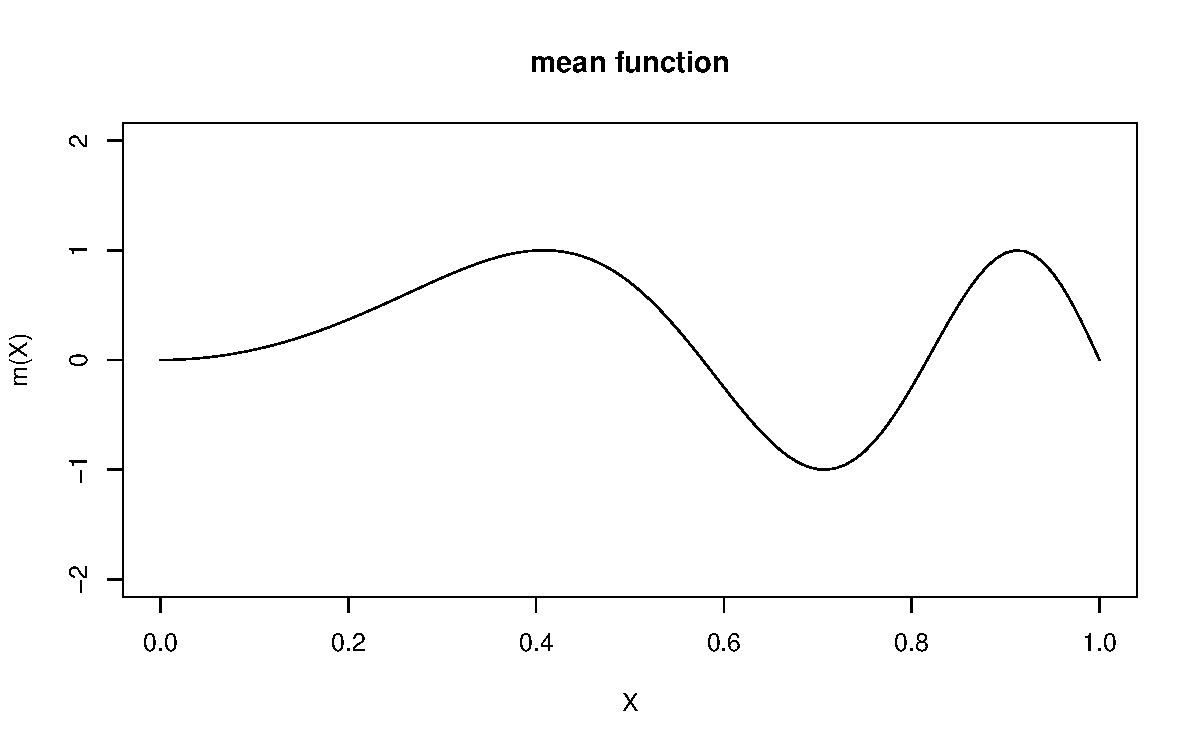
\includegraphics[width=\textwidth]{mfvb_mean.pdf}
        \caption{}
        \label{fig:seq_peak_data}
    \end{subfigure}
    \hfill
    \begin{subfigure}[b]{0.45\textwidth}
        \centering
        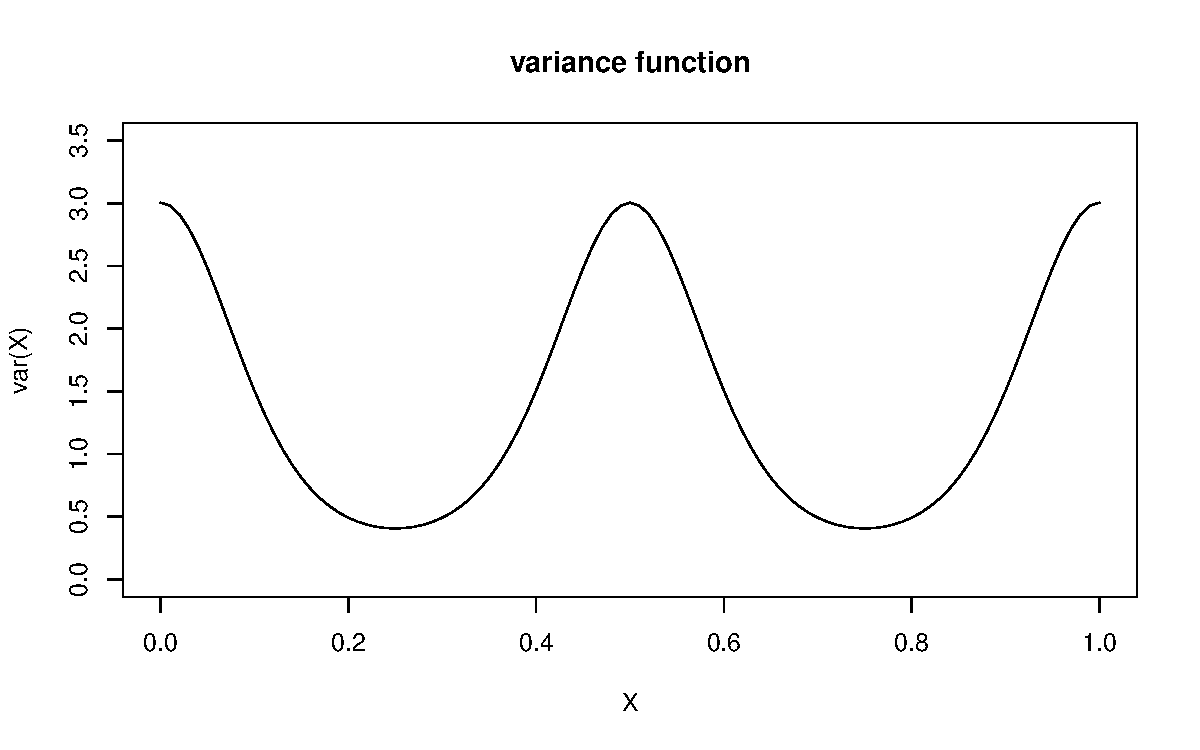
\includegraphics[width=\textwidth]{mfvb_var.pdf}
        \caption{}
        \label{fig:seq_peak_est}
    \end{subfigure}
    \caption{Mean (a) and variance (b) functions used in the simulation study comparing SMASH against MFVB.}
    \label{fig:mfvb_fn}
\end{figure}
In the first scenario, the number of data points is not a power of two, nor are the point equally spaced. To deal with these complications, we adapted and modified the standard symmetric extension procedure commonly adopted in wavelet settings. We first mirrored the data about the right edge and extract the first $2^{\lfloor\log_2(2n)\rfloor}$ sample points. This ensures that the number of data points in the new ``dataset'' is a power of two, and the mean curve would be continuous at the right edge. To further ensure that the input to the Gaussian denoising method is periodic, we then reflected the new dataset about the right edge and used this as the final input. In order to obtain the original mean and variance functions, we extracted the first $n$ points from the outputs (mean and variance) of our denoising technique. Since the data points are not evenly spaced, we took the simplest approach and applied our method treating the observations as if they were evenly spaced. This approach is not only intuitively appealing, but can also be considered a formal treatment of unequally spaced data in traditional wavelet settings (see Sardy et al. (1999)). Evaluation of MSE at the 201 equally spaced points is then based on simple linear interpolation between the estimated points. Tables \ref{table:mfvb_comp} displays the MSEs over 100 independent runs for each scenario.
\begin{table}[ht]
\centering
\begin{tabular}{rrrrr}
\hline
& \multicolumn{2}{c}{Scenario 1}&\multicolumn{2}{c}{Scenario 2}\\
\cline{2-5}
& mean & sd & mean & sd \\
\hline
MFVB & 0.0330 & 0.0199 & 0.0172 & 0.0085 \\
SMASH & 0.0334 & 0.0187 & 0.0158 & 0.0065 \\
\hline
\end{tabular}
\caption{MSEs of MFVB and SMASH for two simulation scenarios}
\label{table:mfvb_comp}
\end{table}
\bigskip\\
Note that wavelets in general are poorly suited for dealing with the setup in Scenario 1; not only are the number of data points not a power of two, they are also not equally spaced. Also, linear interpolation between sample points was used in computing the MSE, further impacting the accuracy of wavelet methods. At the same time, spline-based methods such as MFVB are well suited to dealing with smooth mean and variance functions such as those used in the simulations, whereas wavelet methods can better deal with spatial inhomogeneity which are present in functions such as those presented in Tables
\ref{table:homo1} - \ref{table:hetero_bump_3}. Despite these limitations, our method performs comparably to MFVB in terms of mean estimation for the simulation scheme presented in Scenario 1, and has a lower MSE in terms of variance estimation. For Scenario 2, our method outperforms MFVB in both mean and variance estimation despite the smoothness of the test functions used. \bigskip\\
Summarizing the simulation studies conducted so far, we have demonstrated that our method does a reasonable job of mean and variance estimation for a variety of situations in the Gaussian case. As such, we now turn our attention to the Poisson case. For this simulation study, we considered different test functions and Poisson intensities for a given sample size of $n=1024$ as in Timmermann \& Nowak (1999) and Fryzlewicz \& Nason (2004), over 100 independent runs. Specifically, the ``Spikes'', ``Angles'', ``Bursts'',``Clipped Blocks'',``Bumps'' and ``Heavisine'' functions were chosen. The first 5 were part of a simulation study by Besbeas et al. (2004), and the ``Heavisine'' function was considered by Fryzlewicz \& Nason (2004). These test functions were then shifted and scaled to have (min,max) intensities of (0.01,3), (1/8,8) and (1/128,8), of which the latter two were the values used in Fryzlewicz \& Nason (2004). The low intensity scenario of (0.01,3) was chosen to reflect the small number of counts often present in certain types of high-throughput sequencing data, an application we will demonstrate in more detail later on. To assess the performance of our method, we used the same MISE as defined above for the Gaussian case, and considered the following methods in our simulation study:
\begin{enumerate}
\item SMASH
\item Haar-Fisz transform and variance stabilization (denoted by Haar-Fisz). See Fryzlewicz \& Nason (2004).
\item Anscombe transformation with the universal threshold using hard thresholding (denoted by Anscombe, universal). See Donoho (1993).
\item Anscombe transformation with the cross-validation threshold using hard thresholding (denoted by Anscombe, CV)
\item Corrected Haar thresholds using hard thresholding (denoted by Haar thresholds). See Kolazyk (1997).
\item Conditional variance stabilization with the non-decimated wavelet transform (denoted by CVS). See Jansen (2006).
\item Bayesian multi-scale multiplicative innovations model (denoted by BMMIM). See Timmermann \& Nowak (1999).
\item Bayesian multi-scale model (denoted by BMSM). See Kolaczyk (1999b).
\end{enumerate}
The Haar-Fisz transform uses 50 external cyclespins as suggested by Fryzlewicz \& Nason (2004). The Anscombe transformations use the Symmlet 8 basis, while the Haar-Fisz transformation and CVS use the Symmlet 10 basis, as recommended by the corresponding software. Except for BMSM and our method (which are entirely adaptive), we considered primary resolution levels of 5,6 and 7 for all other methods. We present the MISEs for test functions ``Angles'' and ``Bumps'' in Tables \ref{table:pois_angles} and \ref{table:pois_bumps} respectively; full simulation results can be found in Appendix \ref{}.\bigskip\\
\begin{table}[ht]
\centering
\begin{tabular}{rrrr}
  \hline
 & (0.01,3) & (1/8,8) & (1/128,128) \\
  \hline
SMASH & 145.3 & 68.5 & 10.2 \\
  Haar-Fisz & 369.5 & 140.4 & 9.8 \\
  Anscombe, universal & 459.0 & 163.7 & 10.1 \\
  Anscombe, CV & 458.8 & 162.6 & 10.1 \\
  Haar thresholds & 295.8 & 168.3 & 89.4 \\
  CVS & 5201.1 & 1083.5 & 122.8 \\
  BMMIM & 277.2 & 110.1 & 18.1 \\
  BMSM & 147.4 & 73.9 & 10.5 \\
   \hline
\end{tabular}
\caption{MISEs of various methods for the Angles function for Poisson data}
\label{table:pois_angles}
\end{table}

\begin{table}[ht]
\centering
\begin{tabular}{rrrr}
  \hline
 & (0.01,3) & (1/8,8) & (1/128,128) \\
  \hline
SMASH & 2597.5 & 1194.6 & 141.2 \\
  Haar-Fisz & 2849.9 & 1572.3 & 184.0 \\
  Anscombe, universal & 3500.0 & 2029.9 & 194.9 \\
  Anscombe, CV & 3520.7 & 2070.0 & 196.3 \\
  Haar thresholds & 3151.9 & 1601.4 & 173.7 \\
  CVS & 9410.7 & 3457.5 & 194.9 \\
  BMMIM & 3089.9 & 2065.3 & 222.2 \\
  BMSM & 4036.8 & 1889.9 & 171.1 \\
   \hline
\end{tabular}
\caption{MISEs of various methods for the Bumps function for Poisson data}
\label{table:pois_bumps}
\end{table}

From Tables \ref{table:pois_angles} and \ref{table:pois_bumps} we can see that our method consistently outperforms other methods discussed here. This is particularly evident for the low intensity cases (ie (min,max) intensity of (0.01,3) and (1/8,8)), which are of primary interest in our application to sequencing data. At the same time, our method still performs competitively even when the average/peak intensity is high. Note that our method substantially improves on the performance of other methods for test function ``Bumps'', which is extremely hard to estimate due to its inhomogeneity.

Overall, these simulation studies demonstrate the ability of our method to accurately recover the mean functions for both the Gaussian and Poisson cases, and highlight the flexibility and adaptiveness of the shrinkage procedure ASH. Although we have considered an extensive range of problems here, including different SNRs, sample sizes, variance functions, test functions and mean intensities where applicable, the performance of our method on real data has to be determined. In the next section, we will apply our method to two example datasets that have been discussed in previous work, and comment on the resulting estimates.
\bigskip\\
\section{Application to real datasets}
\subsection{Three-month Treasury Bill Yields}
In this section we apply the Gaussian and Poisson denoising techniques to one example dataset each. For the Gaussian case, we looked at yields of secondary market rates from three-month Treasure bills, which were recorded weekly on Fridays. These rates were quoted on a discount basis and annualized using a 360-day year of bank interest. To match the analysis in Fan \& Yao (1998), we used 1735 weekly observations spanning Jan. 5 1962 to Mar. 31 1995. The data are plotted in Figure \ref{fig:tb_raw_data}. Similar to Fan \& Yao (1998), we fit an autoregressive model of order 5 (AR(5)) to the data and obtained the following:
\begin{eqnarray}
T_t=1.228T_{t-1}-0.234T_{t-2}+0.028T_{t-3}+0.039T_{t-4}-0.066T_{t-5}+Y_t
\end{eqnarray}
where $T_t, t=1,...,1735$ is the time series for the yields, and $Y_t$ are the residuals from fitting the model. Figure \ref{fig:tb_res} shows the plot of $Y_t$ against $X_t\equiv T_{t-1}$. Our goal is to estimate the mean function defined by $E(Y_t|X_t=x)$ as well as the variance function $V(Y_t|X_t=x)$. Note that standard wavelet techniques are not designed for such types of data, where 1) repeated observations are present and 2) the number of data points is not a power of two and the points are unevenly spaced. To tackle the first issue, we use the median of the repeated observations at their respective sample points (see eg Delouille et al. (2004)). Next, we applied the procedure described in the Simulations section when comparing our method against MFVB, which was a modified version of symmetric extension. This deals with the second complication. The estimated mean and conditional variance functions are given in Figures \ref{fig:tb_res} and \ref{fig:tb_var} respectively.\bigskip\\
\begin{figure}[h]
\centering
    \begin{subfigure}[b]{0.4\textwidth}
        \centering
        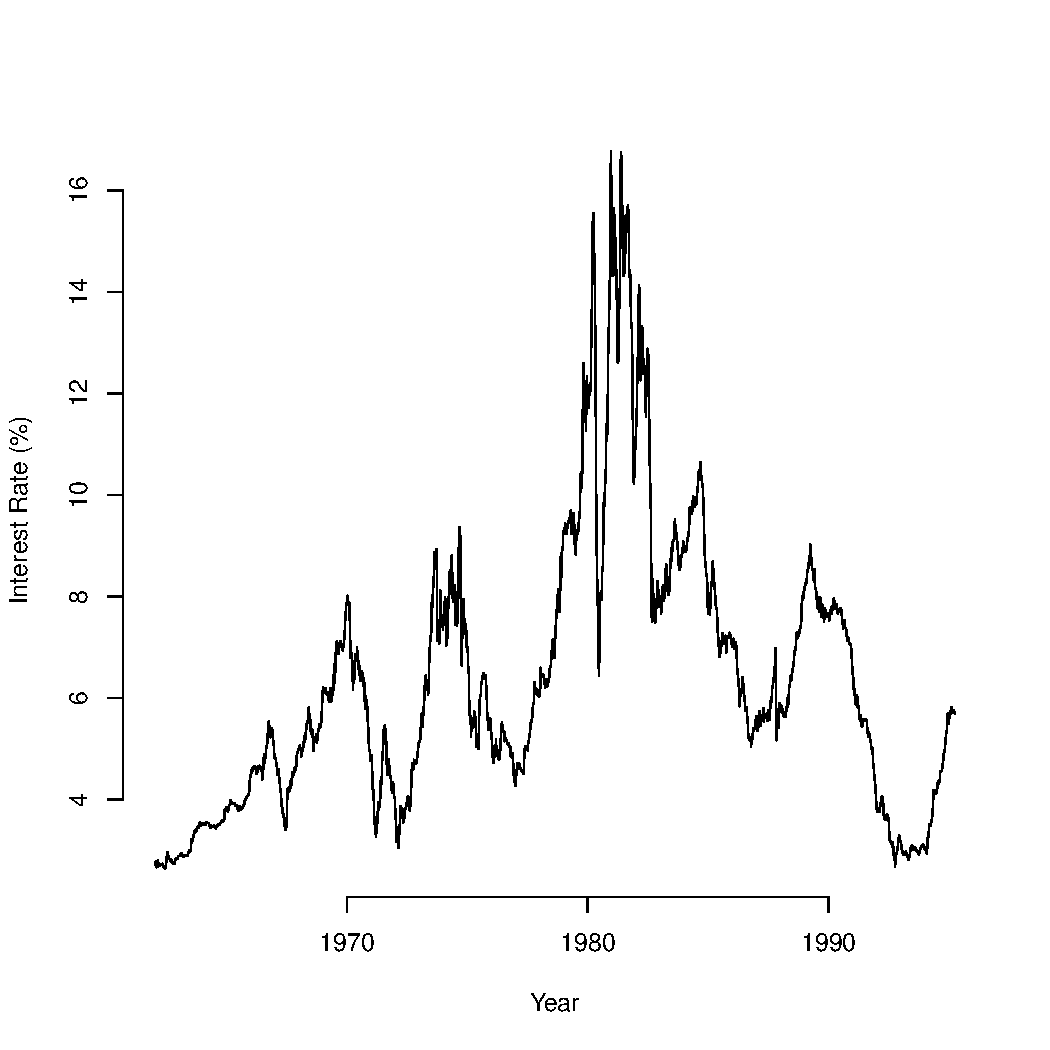
\includegraphics[width=\textwidth]{figures_treasury_a.pdf}
        \caption{}
        \label{fig:tb_raw_data}
    \end{subfigure}
    \hfill
    \begin{subfigure}[b]{0.4\textwidth}
        \centering
        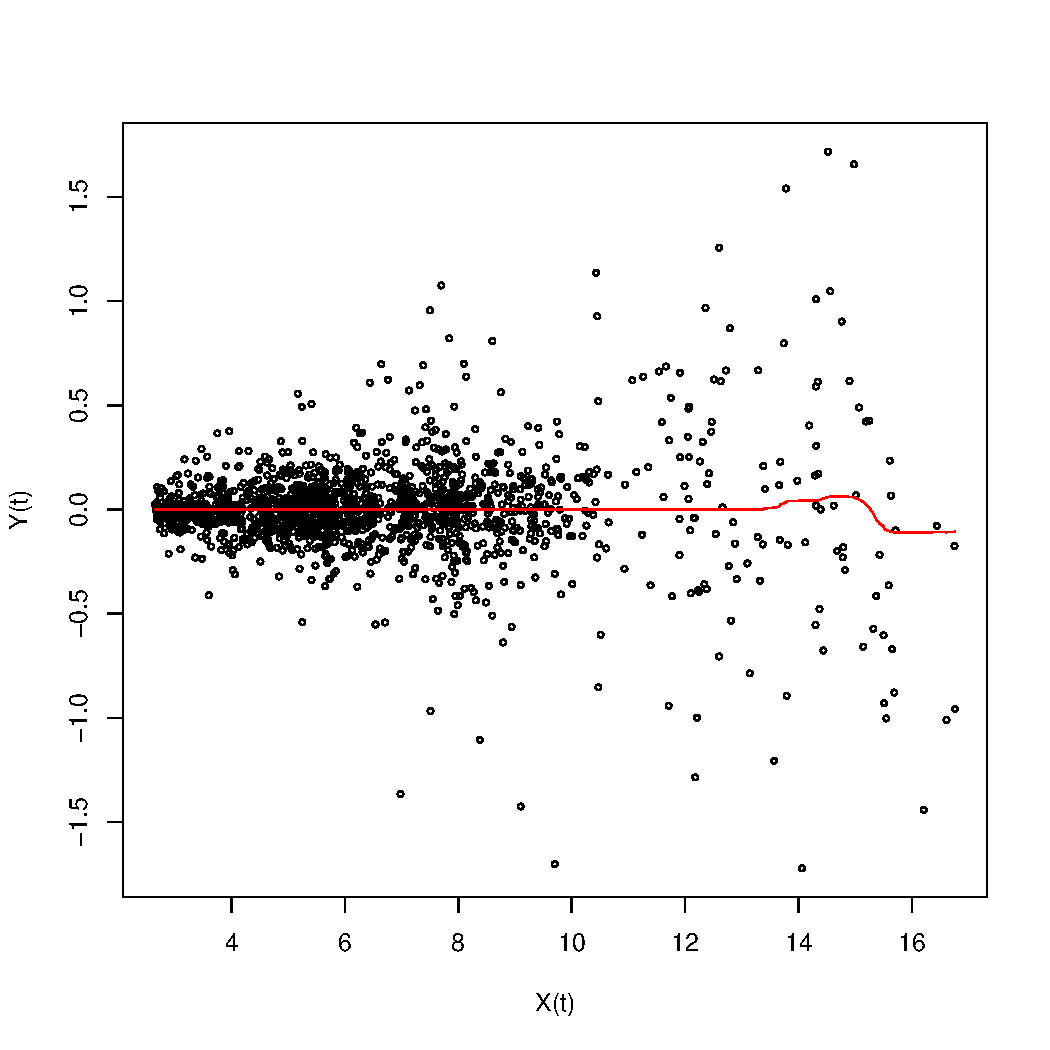
\includegraphics[width=\textwidth]{figures_treasury_b.pdf}
        \caption{}
        \label{fig:tb_res}
    \end{subfigure}

    \begin{subfigure}[b]{0.4\textwidth}
        \centering
        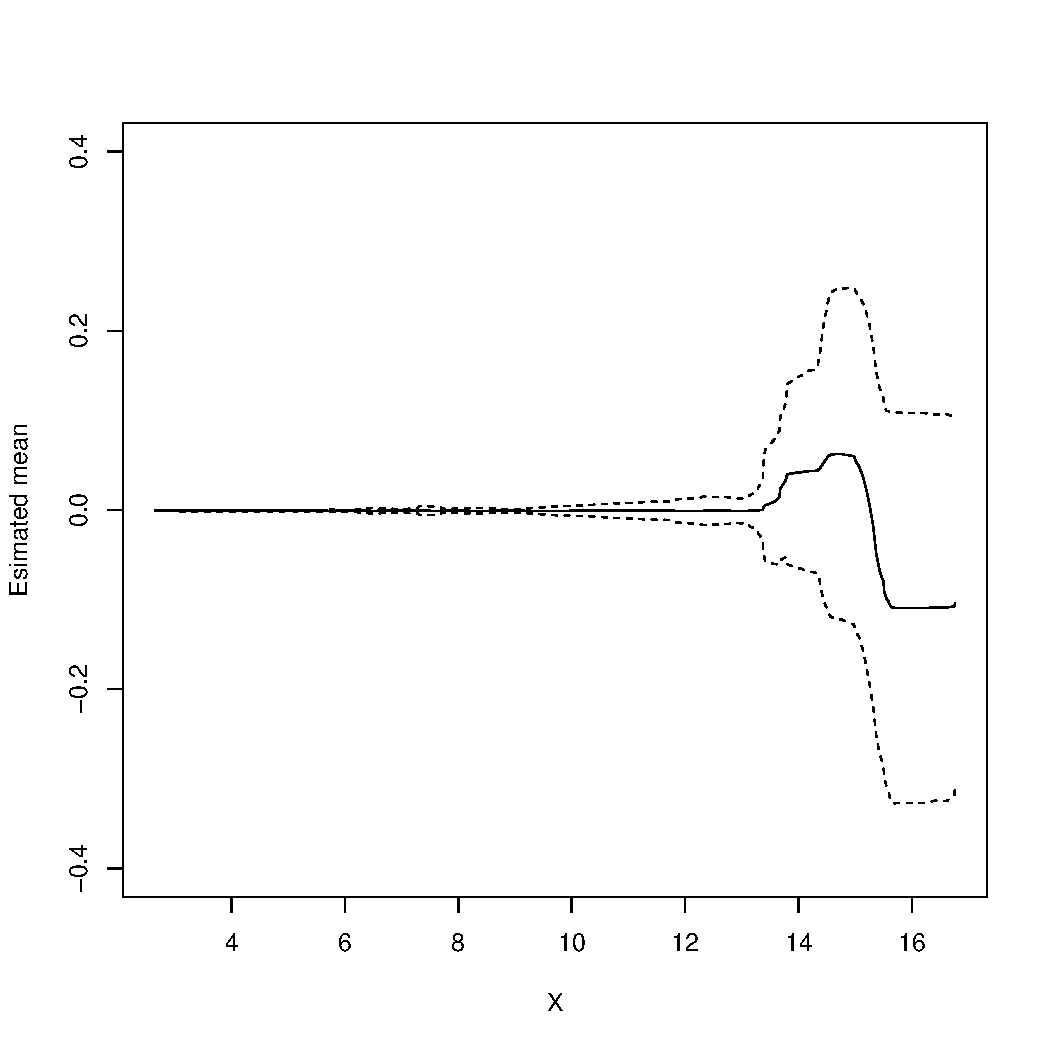
\includegraphics[width=\textwidth]{figures_treasury_c.pdf}
        \caption{}
        \label{fig:tb_mean}
    \end{subfigure}
    \hfill
    \begin{subfigure}[b]{0.4\textwidth}
        \centering
        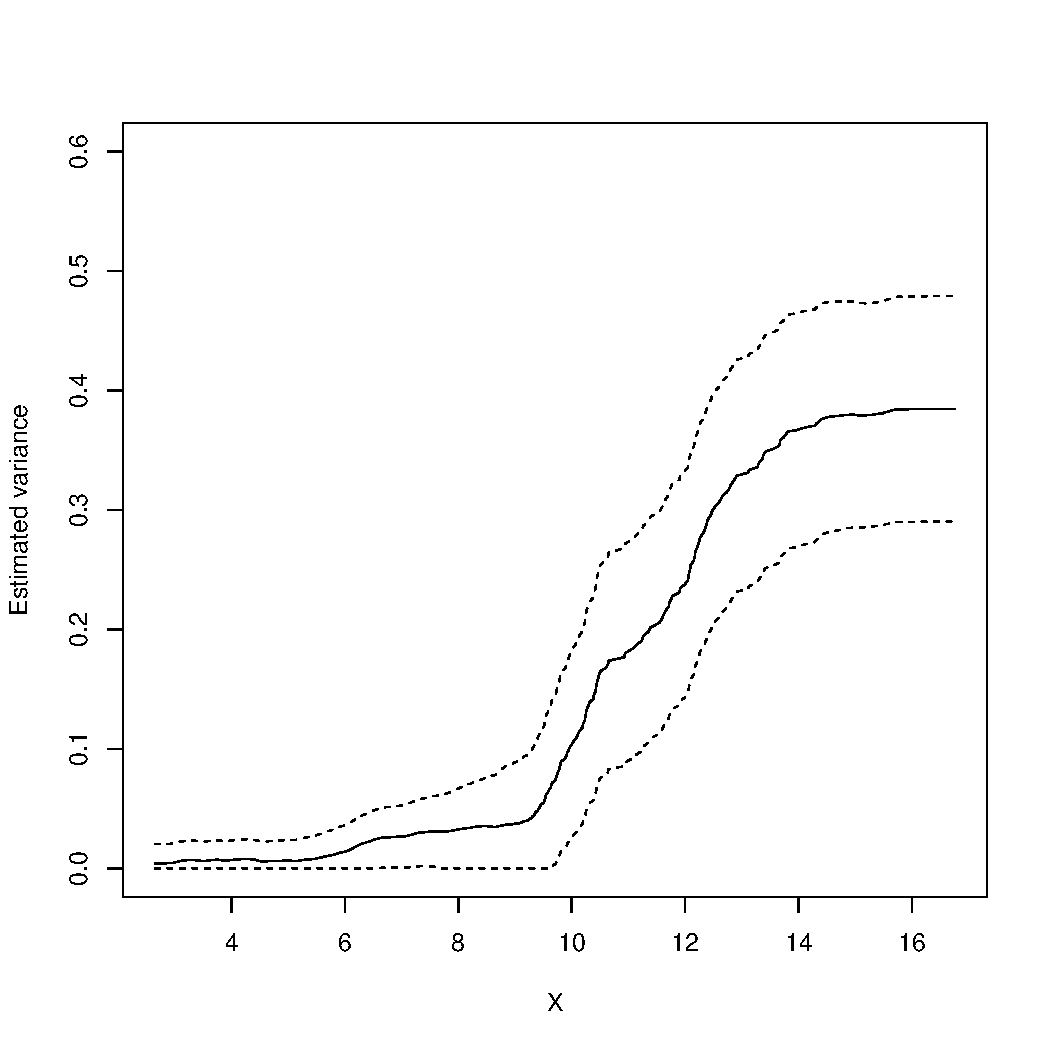
\includegraphics[width=\textwidth]{figures_treasury_d.pdf}
        \caption{}
        \label{fig:tb_var}
    \end{subfigure}
    \caption{Analysis of yields from three-month Treasury Bills. (a) Raw data of interest rates as a function of time. (b) Residuals $Y_t$ from fitting an AR(5) model to the data against $X_t\equiv T_{t-1}$. The red curve is the estimated mean curve from SMASH. (c) Plot of a zoomed-in version of the estimated mean curve, with approximate 95\% credible bands. (d) The estimated conditional variance curve, with approximate 95\% credible bands.}
\end{figure}
\bigskip\\
Except for possible boundary effects, our mean and conditional variance estimates are similar to those of Fan \& Yao (1998). Unfortunately, these boundary effects are difficult to deal with for non-periodic functions in the wavelet case, and our usage of symmetric extension with the Haar basis is just one possible solution. Better alternatives have been suggested by eg. Su et al. (2013), but is beyond the scope of discussion in this paper. Similar to the analysis in Fan \& Yao (1998), we found the correlation coefficient between the logarithm of $x_t$ and the logarithm $\hat{V}^{1/2}(Y_t|x_t)$ to be 0.949, which further supports the structural volatility model suggested by Andersen and Lund (source?):
\begin{eqnarray}
Var^{1/2}(Y_t|x_t)=\Ga x_t^{\Gb}
\end{eqnarray}
By performing least squares regression of $\log(\hat{V}^{1/2}(Y_t|x_t))$ on $\log(x_t)$, we have that $\hat{\Ga}=0.0106$ and $\hat{\Gb}=1.429$, which are similar to the values reported in Fan \& Yao (1998).
\newpage
\subsection{ChIP-Seq Data}
Here we apply our Poisson de-noising procedure to next generation sequencing data, commonly seen in the field of genomics. Specifically, we chose an example dataset from the ENCODE (\textbf{Enc}yclopedia \textbf{O}f \textbf{D}NA \textbf{E}lements) project launched by the National Human Genome Research Institute. This dataset contains reads from chromatin immunoprecipitation sequencing (ChIP-seq) measuring transcription factor binding in two different cell types, with two samples for each cell type. Due to the massive size of the data, we selected a representative portion of the reads of length $2^{15}$ from chromosome 1. Since we are looking mainly at univariate denoising here, we ran our method on each sample separately to produce the the plots in Figure \ref{fig:seq_smooth}.\\
\begin{figure}[h]
\centering
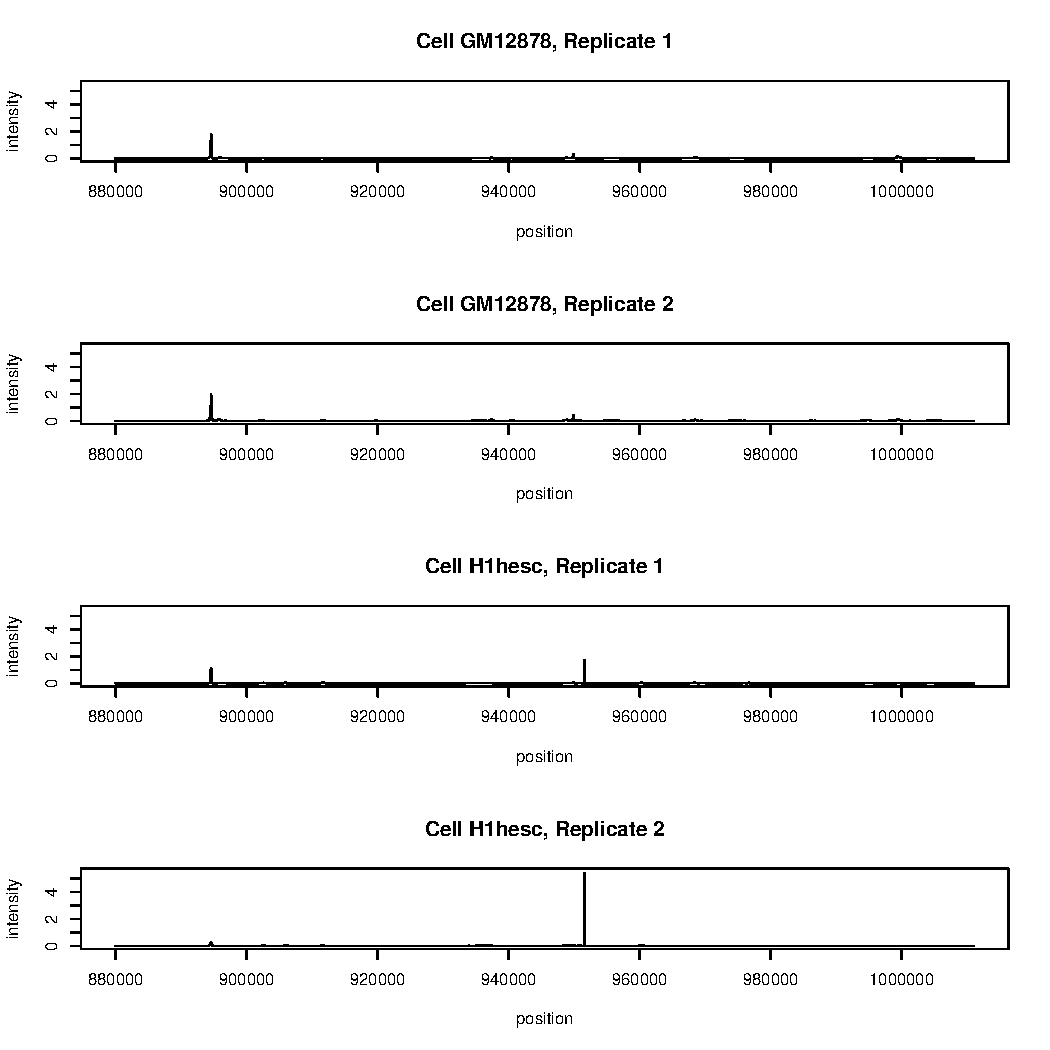
\includegraphics[scale=0.7]{smoothing_all.pdf}
\caption{Estimated intensities from SMASH for 4 samples; the first two samples are two replicates from GM12878, a lymphoblastoid cell line, and the last two samples are two replicates from H1hesc, which are human embryonic stem cells. The reads are taken from position 880001 to 1011072 on chromosome 1.}
\label{fig:seq_smooth}
\end{figure}
\bigskip
One goal of analyzing ChIP-seq data is to discover regions where transcription factors are likely to bind to DNA, thereby allowing us to better understand the mechanisms underlying gene regulation. These binding regions are often reflected in the data as ``peaks'', where more counts are present than background noise. Our method allows us to identify these peaks by looking at the estimated intensity function. In Figure \ref{fig:seq_smooth}, we immediately notice the presence of several large peaks around position 895000 for the first three samples, and around position 952000 for the last two samples. To ensure that our method performs sensibly, we took the same region from only the GM12878 cell line and ran our method as well as a popular peak calling procedure MACS on the region. The results are shown in Figure \ref{fig:seq_peak}.\\
\newpage
\begin{figure}[h]
\centering
    \begin{subfigure}[b]{0.85\textwidth}
        \centering
        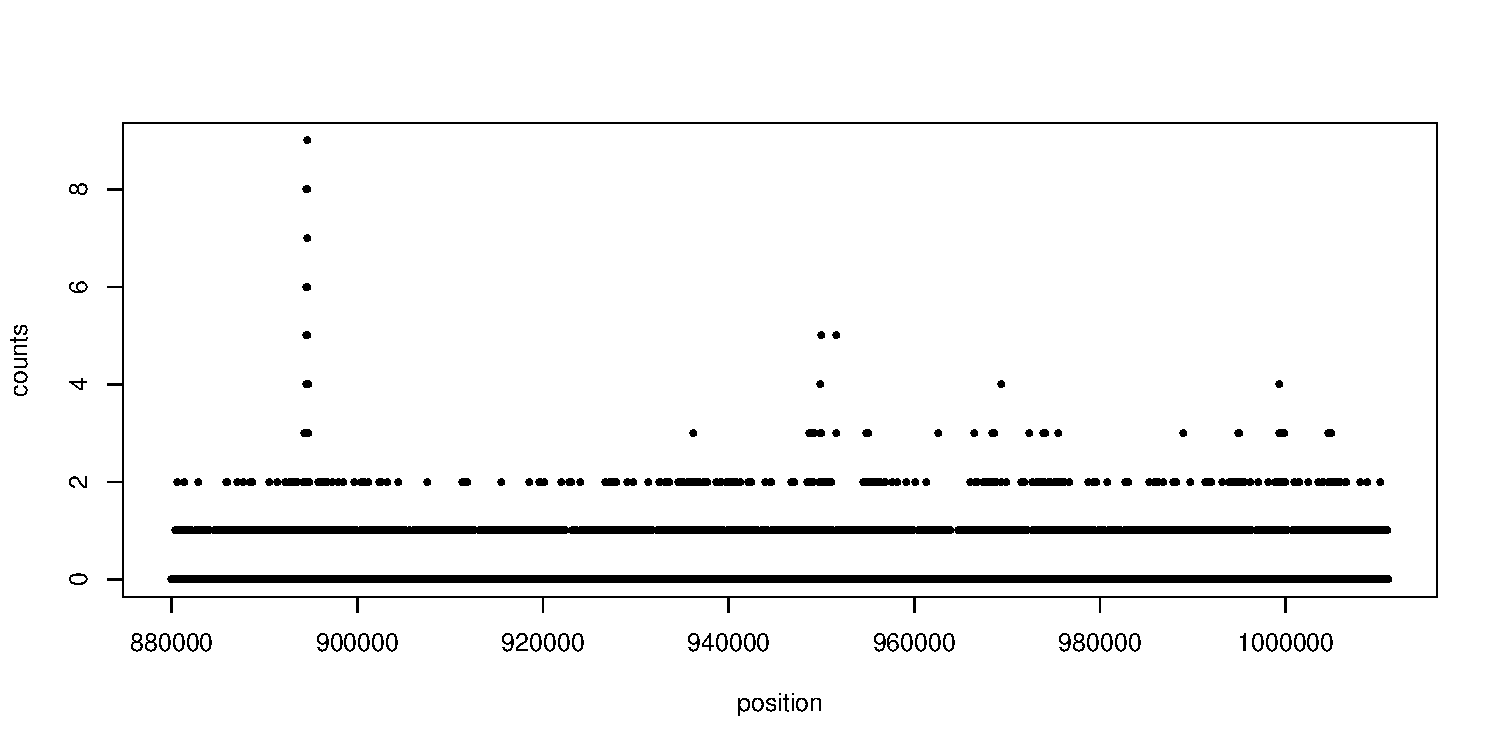
\includegraphics[width=\textwidth]{peaks_comp_a.pdf}
        \caption{}
        \label{fig:seq_peak_data}
    \end{subfigure}

    \begin{subfigure}[b]{0.85\textwidth}
        \centering
        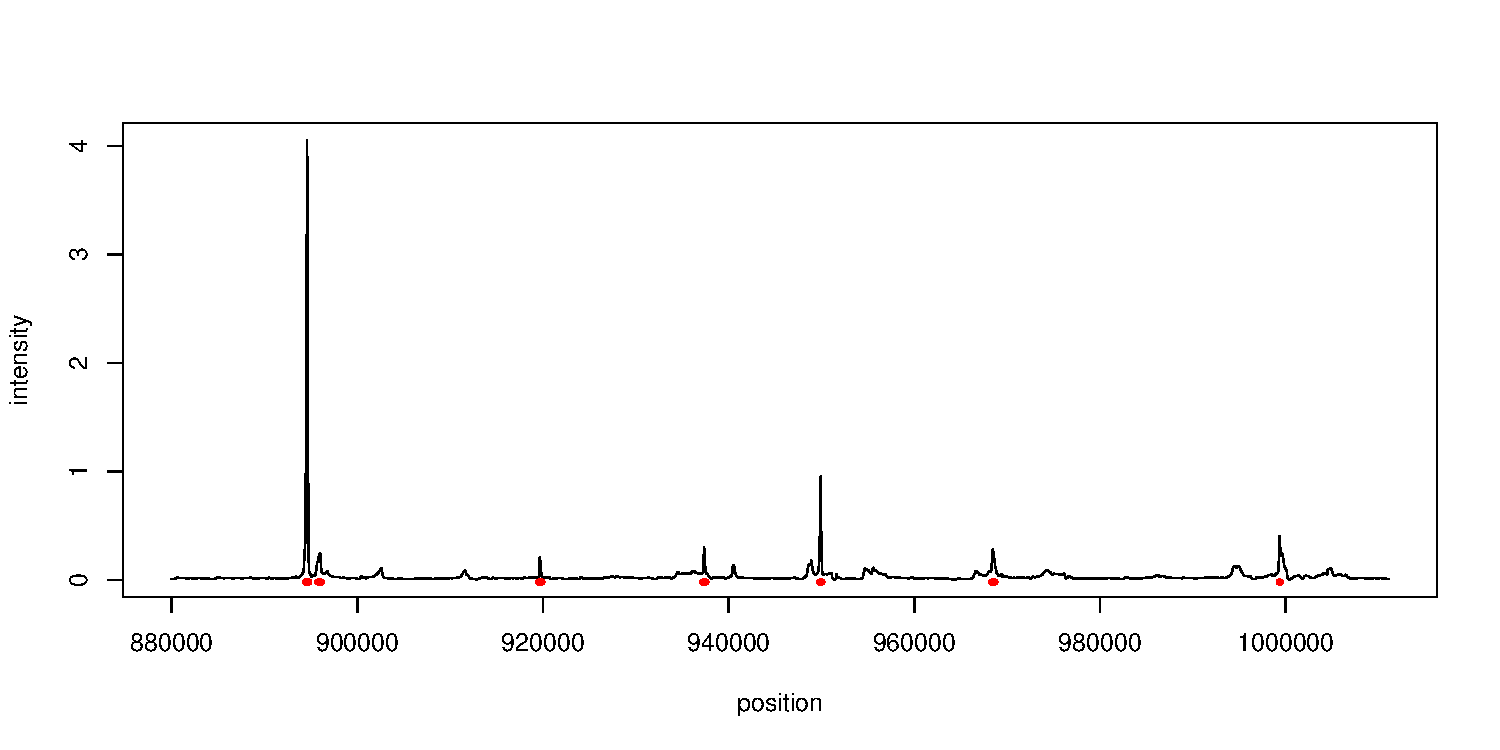
\includegraphics[width=\textwidth]{peaks_comp_b.pdf}
        \caption{}
        \label{fig:seq_peak_est}
    \end{subfigure}
    \caption{Analysis of reads taken from the GM12878 cell line, spanning position 880001 to 1011072 on chromosome 1. (a) Raw sequencing counts. (b) Estimated intensity function from SMASH (black solid line) and location of peaks called by MACS (red markers beneath the estimated intensity).}
    \label{fig:seq_peak}
\end{figure}
From Figure \ref{fig:seq_peak_est} it is clear the intensity estimate from our method can recognize the peaks detected by MACS. Rather than calling peaks based on certain thresholds however, our method allows users to determine the relative strength and width of each peak, which provides a more comprehensive summary of the sequencing reads. At the same time, our method also provides the posterior variances for the intensity estimates, allowing for the option of calling peaks based on thresholds if desired.\\
\section{Discussion}
In this paper we have briefly introduced the adaptive shrinkage method ASH; while it was originally developed in the setting of FDR control for multiple comparisons, we have illustrated its usage as part of two wavelet denoising techniques. Both the applications discussed in this paper relaxes the standard assumption of i.i.d. Gaussian noise, and thus present us with challenging tasks. Through these applications we are able to demonstrate the flexibility and accuracy of the shrinkage method, allowing it to be potentially used in a variety of other applications where shrinkage is desirable.\bigskip\\
In both the aforementioned applications, our software allows users to easily obtain point estimates for the mean function as well as approximate credible intervals to provide uncertainty estimates. In the case of (possibly heteroskedastic) Gaussian errors, we are able to estimate the variance function as well, which can be used to provide frequentist confidence intervals for other forms of mean estimation. To the best of our knowledge, there is no readily available software which implements joint mean and variance estimation in the wavelet literature. We have also tested our method in simulations and found that it is relatively robust to simple forms of autocorrelation between the errors (details needed). In the case of Poisson regression, we have improved upon the conjugate Beta priors used in conjunction with the binomial likelihoods by utilizing ASH as the shrinkage procedure, which allows for more flexibility and precision. In addition, we have proposed a new procedure to assess the performance of a given method on real datasets without knowing the underlying truth, under the assumption that the data follow a Poisson distribution. In both of the applications, one further advantage of both our methods is that there is no tuning parameter other than the type of wavelet basis used. On the other hand, the so-called primary resolution level in almost all of the other wavelet-based methods actually affects their performance substantially, depending on the underlying mean and/or variance function. Hence, our fully adaptive procedures allow users to easily apply them to any given dataset, depending on context.\bigskip\\
We have also demonstrated through numerical studies that our methods mostly outperform their respective counterparts from the standard wavelet literature in terms of pointwise accuracy (MSE in this case). Furthermore, the simplicity of the approximated Gaussian likelihoods as well as the conjugacy of the mixture Gaussians used indicate that our methods are computationally fast, since the posteriors can be computed analytically. In the Gaussian case, the only available method (which we implemented ourselves) for mean estimation with heteroskedastic errors is a non-Bayesian thresholding procedure, making it difficult to assess the relative computational efficiency of our method. Furthermore, the lack of readily available software for variance estimation made it extremely difficult to assess the relative performance of our method in that context as well. On the other hand, we were able to compare our method to some of the more popular denoising techniques in the Poisson case. Specifically, we have improved upon the conjugate Beta priors used in conjunction with the binomial likelihoods (Kolaczyk 1999) by utilizing ASH as the shrinkage procedure, which allows for more flexibility and accuracy. This is particularly evident in the case where the mean intensity is low, as is common in many high-throughput genomic sequencing datasets. Our method is also much faster and comparable in accuracy to the popular Haar-Fisz algorithm, due to the fact that we do not have to perform external cycle-spinning. Unfortunately, we were not able to directly compare the computational efficiency of our method to other methods due to differences in the programming software involved including that of the multiscale approach from Kolaczyk (1999).\bigskip\\
Although we have only focused on one-dimensional univariate denoising here, our methods can be extended to various scenarios. Even while restricting ourselves to the one-dimensional domain, our methods could be used in the case of multiple samples, otherwise known as regression analysis of functional data (see Morris 2006). Instead of dealing with a vector of observations, we could perform regression analysis on a matrix of observations, each row of which would encapsulate a sample with observations that are temporally or spatially structured. While Morris (2006) proposed a way to solve a generic regression model, they implicitly assumed the same variance structure for each sample in the same group or category. Our work in the Gaussian case potentially allows for differing variance structures amongst all the samples, thereby imposing even less restrictions on the assumptions behind the regression model. In the simplest case, we could potentially obtain spatially structured differences between the samples by including a single covariate into the regression model that categorizes each sample. In particular, the Poisson model is extremely useful for discovering regions in sequencing reads where differential expression is present between say, different tissues, as per our sequencing example in the previous section. The Gaussian model could potentially be used in...(??).\bigskip\\
With some work, our methods could also be extended to higher dimensions, where a wider range of applications is possible. For example, we could attempt a straight extension to the two dimensional case for both the Gaussian and the Poisson cases as described in Nowak (1998) (again, reference technical report). However, recent advances in image denoising problems have shown that wavelet transformations might not be the most ideal due to the presence of smooth curves in many images such as photographs. We could thus attempt to use ASH as a shrinkage procedure in other types of transformations such as curvelets, and that could be a potential direction for future work.
\newpage
\section{Reference}

\begin{appendices}
\section{}\label{app:var estimation}\bigskip
\textbf{Variance estimation for Gaussian denoising}\bigskip\\
With $\bm{Z}$ as defined in \eqref{eq:varobs1}, we apply the wavelet transform $W$ to $\bm{Z}^2$, and obtain the wavelet coefficients $\bm{\Gd}=W\bm{Z}^2$. Note that $\mathbb{E}(\bm{\Gd})=(\bm{\Gg})$, where $\bm{\Gg}=W\bm{\s}^2$. As with \eqref{eq:likelihood}, we treat the likelihood for $\bm{\Gg}$ as if it were independent, resulting in
\begin{eqnarray}
L(\bm{\Gg}|\bm{\Gd})=\prod_{j=0}^J\prod_{k=0}^{T-1}P(\Gd_{jk}|\Gg_{jk})
\end{eqnarray}
However, the likelihoods $L(\Gg_{jk}|\Gd_{jk})$ are not normal, and have no simple closed form expressions. As such, we approximate the likelihood by a normal likelihood through matching the moments of a normal distribution to the distribution $P(\Gd_{jk}|\Gg_{jk})$ i.e.
\begin{eqnarray}
P(\Gd_{jk}|\Gg_{jk})\approx N(\Gg_{jk},\hat{\mathbb{V}}(\Gd_{jk}))
\end{eqnarray}
so that
\begin{eqnarray}\label{eq:gaus approx}
L(\Gg_{jk}|\Gd_{jk})\approx \phi(\Gd_{jk};\Gg_{jk},\mathbb{V}(\Gd_{jk}))
\end{eqnarray}
where $\phi$ is the normal density function, and $\mathbb{V}(\Gd_{jk})$ is the variance of the detail coefficients. Since these variances are unknown, we estimate them from the data and then proceed to treat them as known. More specifically, since $Z_i\sim N(0,\s_i^2)$, we have that
\begin{eqnarray}
&\mathbb{E}(Z_i^4)\approx 3\s_i^4\notag\\
\label{eq:varvarest}\Rightarrow&\mathbb{V}(Z_i^2)\approx 2\s_i^4
\end{eqnarray}
and so we simply use $\frac{2}{3}Z_i^4$ as an unbiased estimator for $\mathbb{V}(Z_i^2)$. It then follows that $\hat{\mathbb{V}}(\Gd_{jk})$ is given by $\sum_{l=1}^n \frac{2}{3}Z_l^4W_{jk,l}^2$, and is unbiased for $\mathbb{V}(\Gd_{jk})$. These will be the inputs to ASH, which then produces shrunk estimates in the form of posterior means for the corresponding parameters. Although this works well in most cases, there are variance functions for which the above procedure tends to overshrink the detail coefficients at the finer levels. This is likely due to the fact that the distribution of the wavelet coefficients are extremely skewed, especially when the true coefficients are large (at coarser levels the distributions are much less skewed since we are dealing a linear combination of a large number of data points). One way around this issue is to employ a procedure that jointly shrinks the coefficients $\bm{\Gg}$ and their variance estimates (see JASH). The final estimate of the variance function is obtained from the posterior means via the average basis inverse across all the shifts.\bigskip\\

\section{}\label{app:reconstruction}\bigskip
\textbf{Signal reconstruction for Poisson denoising}\bigskip\\
Given the posterior means and variances of the $\Ga$'s from ASH, the first step to reconstructing the signal is to find the posterior means of $p_{jk}:=\frac{\Gl_{j+1,2k}}{\Gl_{jk}}$ and $q_{jk}:=\frac{\Gl_{j+1,2k+1}}{\Gl_{jk}}$ (for $j=0,...,J-1$ and $k=0,...,2^j-1$). Specifically, for each $j$ and $k$, we wish to find
\begin{eqnarray}\label{eq:pfromwc1}
&&E(p_{jk})\equiv E\left(\frac{e^{\Ga_{jk}}}{1+e^{\Ga_{jk}}}\right)\\
\label{eq:pfromwc2}&&E(q_{jk})\equiv E\left(\frac{e^{-\Ga_{jk}}}{1+e^{-\Ga_{jk}}}\right)\end{eqnarray}
Given that we already have the posterior expectations and variances for $\Ga_{jk}$, we can approximate \eqref{eq:pfromwc1}-\eqref{eq:pfromwc2} using the Delta method. First, define
\begin{eqnarray}\label{eq:ff}ff(x)=\frac{e^x}{1+e^x}\end{eqnarray}
and consider the Taylor expansion of $ff(x)$ about $ff(E(x))$:
\begin{eqnarray}\label{eq:delta}ff(x)\approx ff(E(x))+ff'(E(x))(x-E(x))+\frac{ff''(E(x))}{2}(x-E(x))^2\end{eqnarray}
where
\begin{eqnarray}
\label{eq:fderiv}&&ff'(x)=\frac{e^x}{(1+e^x)^2}\\
\label{eq:sderiv}&&ff''(x)=\frac{e^x(1-e^{x})}{(1+e^x)^3}
\end{eqnarray}
It is easy to see that
\begin{eqnarray}
&&E(p_{jk})\approx ff(E(\Ga_{jk}))+\frac{ff''(E(\Ga_{jk}))}{2}Var(\Ga_{jk})\\
\label{eq:Ep}&&E(q_{jk})\approx ff(-E(\Ga_{jk}))+\frac{ff''(-E(\Ga_{jk}))}{2}Var(\Ga_{jk})
\end{eqnarray}
noting that we have already computed $E(\Ga)$ and $Var(\Ga)$.\bigskip\\
Finally, we can easily back-transform to construct an estimated signal, by noting that we can express $\Gl_i$ as a product of the $p$'s and $q$'s for any $i=1,2,...,n$. Specifically, let $\{c_1,...,c_J\}$ be the binary representation of $i-1$, and $d_m=\sum_{j=1}^m c_j2^{m-j}$ for $j=1,...,J-1$. We then have
\begin{eqnarray}\label{eq:product}\Gl_k=\Gl_{00}p_{00}^{1-c_1}p_{1,d_1}^{1-c_2}...p_{J-1,d_{J-1}}^{1-c_J}q_{00}^{c_1}q_{1,d_1}^{c_2}...q_{J-1,d_{J-1}}^{c_J}\end{eqnarray}
where we usually estimate $\Gl_{00}$ by $\sum_l Y_l$ (see Kolaczyk (1999)). Using the independence of the $p$'s and $q$'s from different scales, we have:
\begin{eqnarray}\label{eq:Eproduct}E(\Gl_i)=\Gl_{00}E(p_{00})^{1-c_1}E(p_{1,d_1})^{1-c_2}...E(p_{J-1,d_{J-1}})^{1-c_J}\notag\\
E(q_{00})^{c_1}E(q_{1,d_1})^{c_2}...E(q_{J-1,d_{J-1}})^{c_J}\end{eqnarray}
\bigskip\\
As an additional step, we can also construct a credible band around the signal using the posterior variances for inference purposes. From \eqref{eq:product} we have the following:
\begin{eqnarray}\label{eq:E2product}E(\Gl_i^2)=\Gl_{00}^2E(p_{00}^2)^{1-c_1}E(p_{1,d_1}^2)^{1-c_2}...E(p_{J-1,d_{J-1}}^2)^{1-c_J}\notag\\
E(q_{00}^2)^{c_1}E(q_{1,d_1}^2)^{c_2}...E(q_{J-1,d_{J-1}}^2)^{c_J}\end{eqnarray}
To compute the terms in \eqref{eq:E2product}, we again make use of the Delta method (with $ff(x)=(\frac{e^x}{1+e^x})^2$) to obtain:
\begin{eqnarray}
&E(p_{jk}^2)\approx \left(ff(E(\Ga_{jk}))+\frac{ff''(E(\Ga_{jk}))}{2}Var(\Ga_{jk})\right)^2+\notag\\
& \hspace{1.5 in}\{ff'(E(\Ga_{jk}))\}^2Var(\Ga_{jk})\\
&E(q_{jk}^2)\approx \left(ff(-E(\Ga_{jk}))+\frac{ff''(-E(\Ga_{jk}))}{2}Var(\Ga_{jk})\right)^2+\notag\\
& \hspace{1.5 in}\{ff'(E(-\Ga_{jk}))\}^2Var(\Ga_{jk})
\end{eqnarray}
Finally we combine \eqref{eq:Eproduct} and \eqref{eq:E2product} to find $Var(\Gl_k)$, which allows us to construct credible intervals.\bigskip\\
Note here that in order for the reconstructed signal to possess the property of shift invariance (see Coifman \& Donoho (1995)), the $\Ga$'s are extracted from a so-called translation invariant (TI) table (see Coifman \& Donoho (1995), and Kolaczyk (1999)) rather than as described above. The idea remains the same however, and we can simply think of the extra $\Ga$'s as being defined similarly as the original $\Ga$'s, albeit from a shifted version of the original data points. To be more specific, the TI table contains the $\Ga_{jk}$ for all circulant shifts of the signal. Here we define the $t$-th shift of the signal $\bm{Y}$, denoted by $\bm{Y}^{(t)}$, to be created from $\bm{Y}$ itself by moving the first $n-t$ elements of $\bm{Y}$ $t$ positions to the right and then putting the last $t$ elements of $\bm{Y}$ in the first $t$ locations. Using this table, we are essentially computing the posterior expectations in \eqref{eq:Eproduct}-\eqref{eq:E2product} by averaging over all posterior expectations for every shift of the original signal ie.
\begin{eqnarray}
\label{eq:TIapproxexp}\frac{1}{n}\sum_{t=1}^n E(\hat{\Gl}_k^{(t)})
\end{eqnarray}
which is an approximation to the true quantity we wish to compute, given by
\begin{eqnarray}
E(\hat{\Gl}_k)=\sum_{t=1}^n E(\hat{\Gl}_k^{(t)})P(\mbox{$t$-th shift})
\end{eqnarray}
\end{appendices}
\end{document}
